\documentclass[12pt]{article}
\usepackage{pagecolor,lipsum}
\usepackage{graphicx}
\usepackage{authblk}
\usepackage{setspace}
\usepackage{mathtools}
\usepackage{verbatim}
\usepackage{array}
\usepackage{fancyhdr}
\usepackage{chngcntr}
\usepackage{secdot}
\usepackage{listings}
\usepackage{titling}
%\usepackage[dvipsnames]{xcolor}
\sectiondot{subsection}
\setlength{\parindent}{0cm}
\counterwithout{subsection}{section}
\usepackage{courier}
\lstset{basicstyle=\ttfamily}
\newcommand*{\rom}[1]{\expandafter\@slowromancap\romannumeral #1@}
\usepackage[left=2cm, top=2cm, text={17cm, 24cm}]{geometry}
\usepackage[%  
    colorlinks=true,
    pdfborder={0 0 0},
    linkcolor=blue
]{hyperref}
\definecolor{comment}{rgb}{0.16, 0.5, 0.1}
\definecolor{keyw}{rgb}{0.50, 0.20, 0.9}

\onehalfspacing
\pagestyle{fancy}
\fancyhf{}
\chead{\thepage}
\renewcommand{\headrulewidth}{0.5pt}

\newcommand{\subtitle}[1]{%
  \posttitle{%
    \par\end{center}
    \begin{center}\large#1\end{center}
    \vskip0.5em}%
}
%%%%%%%%%%%%%%%%%%% TITLE PAGE %%%%%%%%%%%%%
\title{

\includegraphics[scale=0.7]{logo (1).png}\\
\huge{5. část - Dokumentace popisující finální schéma databáze}
}
\subtitle{27. Internetový obchod s pastelkami a skicáky}
\author{Verevkin Aleksandr (xverev00)\\
        Tsiareshkin Ivan (xtsiar00)}
\date{02.05.2022}
\newpage

\begin{document}
\pagecolor{white}
\maketitle
\thispagestyle{empty}
\newpage

\section*{Zádaní}
    \indent Cílem je vytvoření jednoduché aplikace pro internetový obchod s pastelkami
    a skicáky. Návštěvníci si mohou pomocí internetového rozhraní prohlížet veškerý 
    sortiment obchodu. Pastelky mohou lišit podle typu (obyčejné, progresso,
    voskovky, ...) a délky, počtu pastelek v balení, atd. Skicáky se dělí podle gramáže, velikosti, počtu papírů, apod. Pokud má návštěvník zájem o určitý produkt/y, 
    může si jej vybrat (vložením do nákupního košíku). U registrovaných zákazníků, kteří jsou do systému přihlášeni, zůstává informace o vybraném zboží v košíku uložena a 
    při opětovném přihlášení znovu načtena. Zákazník si může zboží objednat po zadání potřebných údajů (kontakt, doprava, ...). Zákazníci mohou jednotlivé zboží hodnotit 
    a psát na něj recenze. V systému jsou uloženy také základní údaje o dodavatelích pro opětovné přiobjednání dalšího zboží. Zaměstnanci mohou nahlédnout do statistik oblíbenosti a prodejnosti zboží.
    
\section*{Schéma databáze}
    \begin{center}
        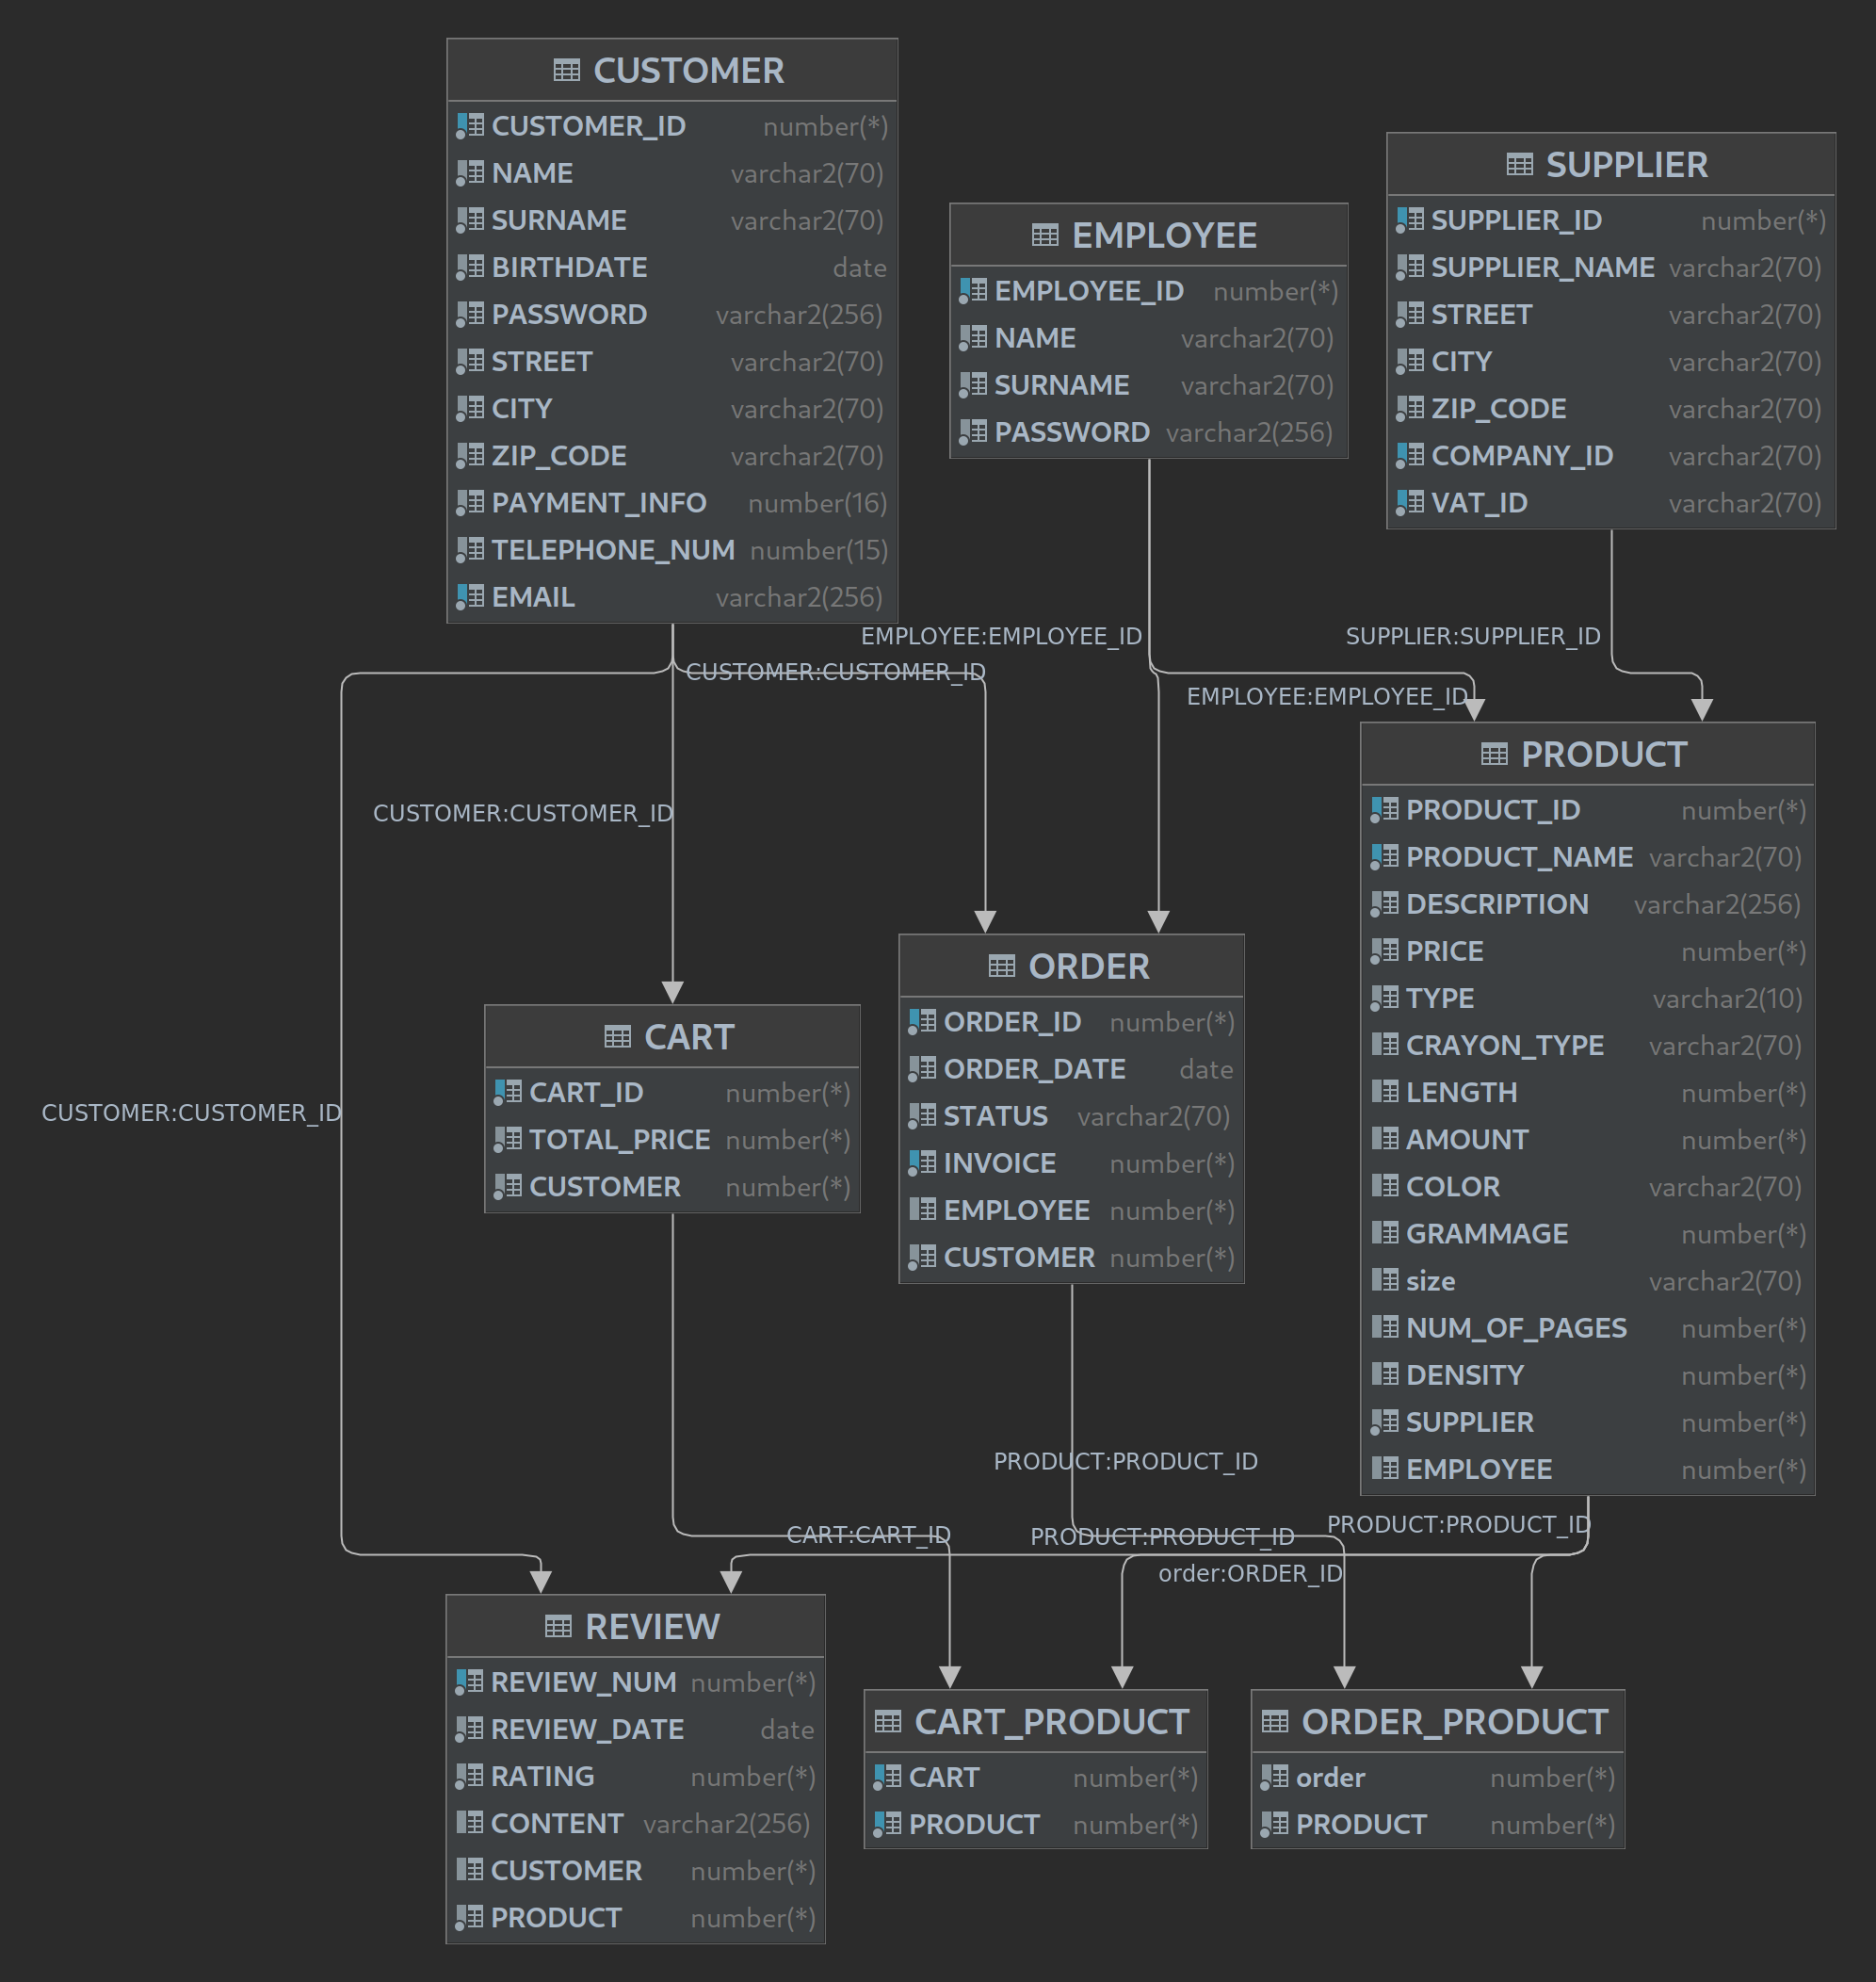
\includegraphics[scale=0.19]{11.png}
    \end{center}
    
\section*{1. Způsob převodu generalizace do schéma relační databáze}
    Produktem může být pastelka nebo skicák, použili jsme jednu tabulku pro uložení
    obou typu produktu. Tabulka \texttt{product} obsahuje atribut \texttt{type}, který definuje typ produktu, a také všechny nutné atributy pastelky a skicáku, které jsou zpočátku nastaveny na \texttt{NULL}.

    \begin{center}
        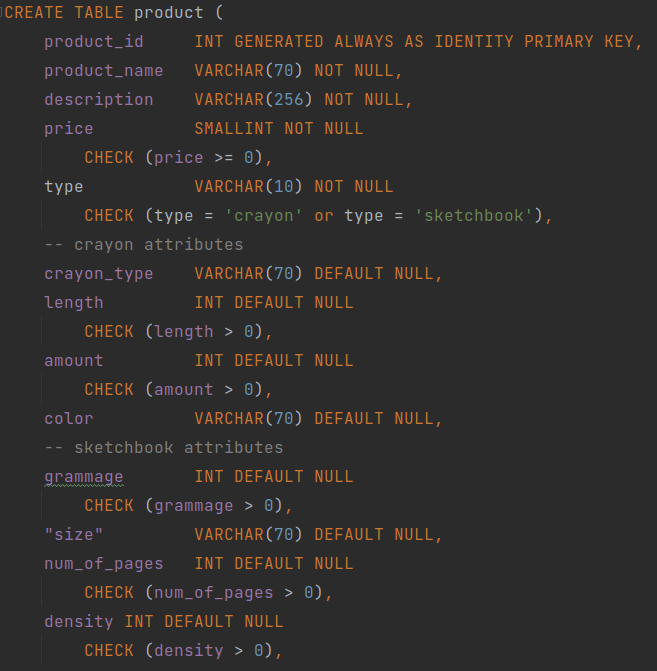
\includegraphics[scale=0.45]{10.png}
    \end{center}

\section*{2. Triggery}
\begin{itemize}
    \item První trigger slouží k aktualizaci celkové ceny nákupního košíku. Spouští se před každým vložením do košiku nových produktů. V cyklu se vypočítá celková cena košíku, přidá se cena nového produktu a aktualizuje se cena košíku.
\end{itemize}
    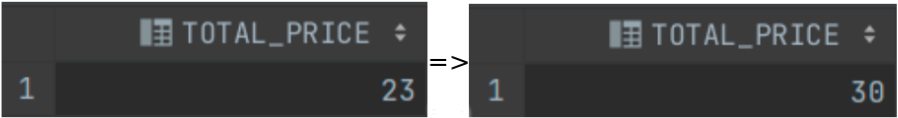
\includegraphics[scale=0.54]{1-2.png}
\newpage
\begin{itemize}
    \item Druhý trigger spouští před vložením nové recenze. Zkontroluje, zda tento uživatel již má recenzi na tento produkt, pokud recenze již existuje, vypíše chybu.
\end{itemize}

\includegraphics[scale=0.6075]{3.png}


\section*{3. Procedury}
\begin{itemize}
    \item První procedura zobrazuje objednávky, které jsou na cestě a zaměstnance odpovědné za jejich doručení. Pokud je v objednávce 0 produktů, vypíše se chyba. Procedura deklaruje kurzor s příkazy, iteruje přes atributy příkazu v cyklu a vypisuje je.
\end{itemize}
    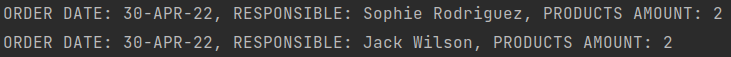
\includegraphics[scale=0.66]{4.png}
\begin{itemize}
    \item Druhá procedura vezme název produktu jako argument a vytiskne jeho dodavatele.
    \begin{center}
        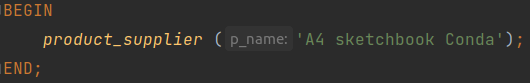
\includegraphics[scale=0.66]{5.png}
        
\includegraphics[scale=0.825]{6.png}
    \end{center}
\end{itemize}

 \section*{4. Přístupová práva}
    Přístupová práva byla předana postupně pomocí příkazu \texttt{GRANT ALL} pro databázové \mbox{tabulky} a \texttt{GRANT EXECUTE} pro procedury.

\section*{5. Explain plan}
    EXPLAIN PLAN se spouští dvakrát pro stejný select, který zobrazuje množství recenzí pro každý produkt.
    \newpage
    \begin{itemize}
        \item Po spuštění EXPLAIN PLAN, je vidět provedené operace, jejich cenu a čas.
        \small
    \end{itemize}
        \begin{center}
            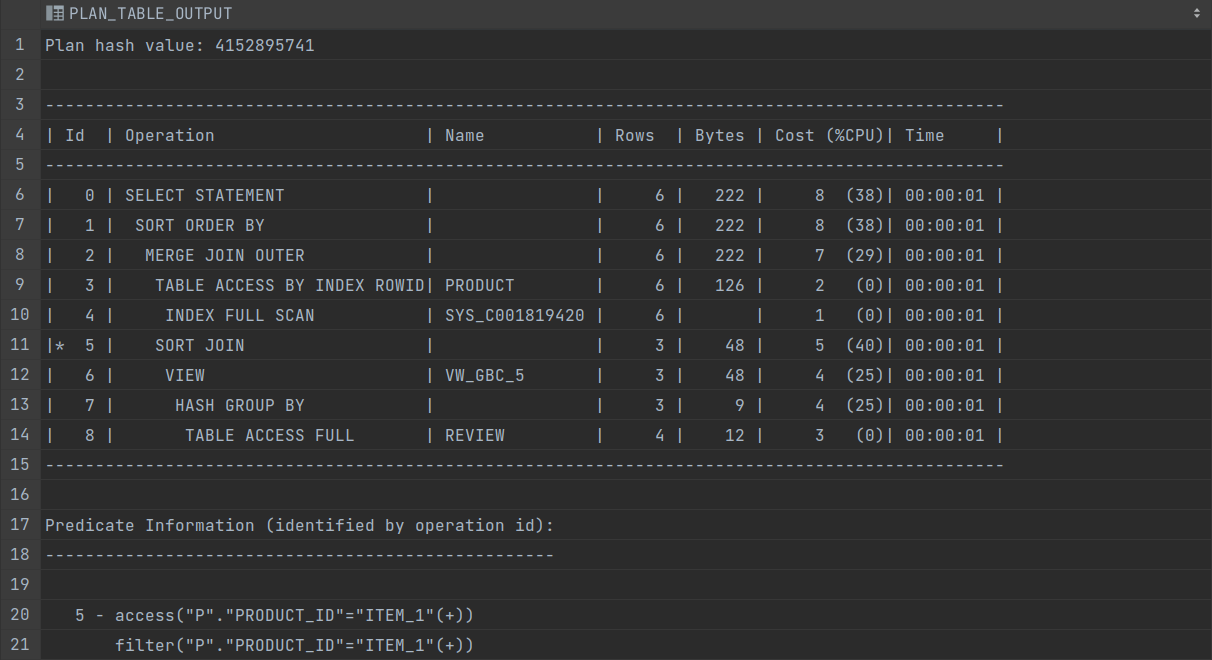
\includegraphics[scale=0.38]{7.png}
        \end{center}
    \begin{itemize}
        \item Pro zrychlení selectu a snížení ceny byl vytvořen index \texttt{product indentif}, který obsahuje id produktu a jeho název. Po spuštění EXPLAIN PLAN je vidět, že select neprochází celou tabulku a používá index, což urychluje vyhledávací operace.
    \end{itemize}
    \begin{center}
        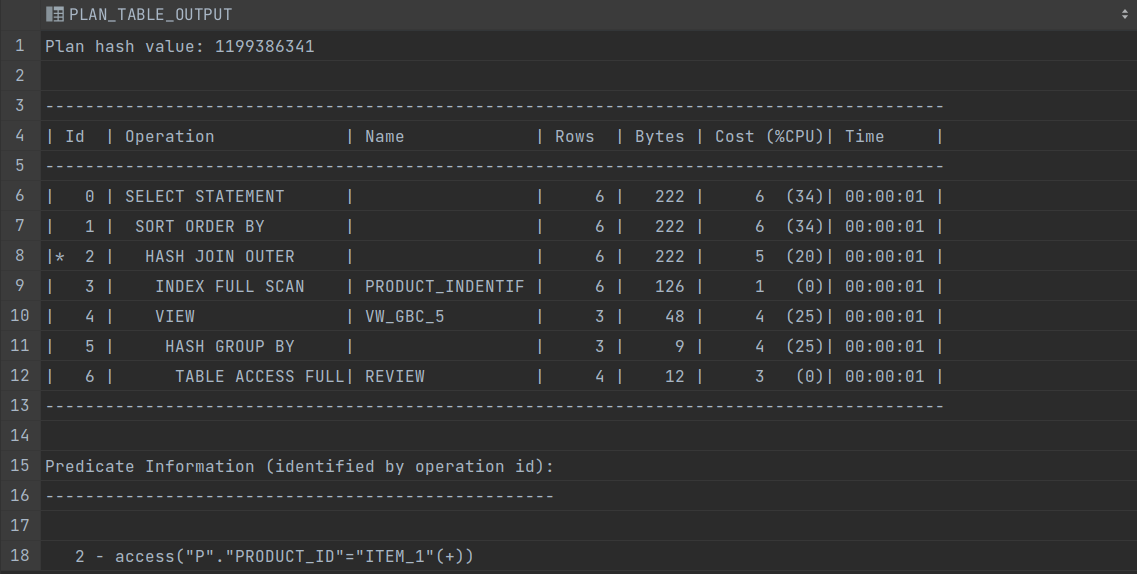
\includegraphics[scale=0.405]{8.png}
    \end{center}
 
\newpage
\section*{6. Materializovaný pohled}
\indent Materializovaný pohled byl vytvořen s produkty a jejich dodavateli. Pohled je uložen v paměti a při přidávání nových produktů se nemění, takže stav tabulky je uložen pro případné další použití.
    
    \begin{center}
        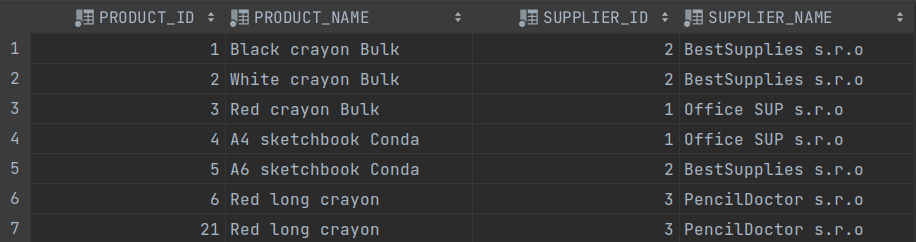
\includegraphics[scale=0.4936]{9.png}
    \end{center}

    Materializovaný pohled patří druhému členu týmu (xtsiar00) a používá tabulky definované prvním členem týmu (xverev00).
\end{document}
